% !TEX program = xelatex
% 编译方式：xelatex report.tex（需安装 ctex 宏包，支持中文）
\documentclass[11pt,a4paper]{ctexart}

\usepackage{geometry}
\geometry{margin=2.5cm}
\usepackage{graphicx}
\usepackage{booktabs}
\usepackage{amsmath,amssymb}
\usepackage{caption}
\usepackage{float}
\usepackage{array}
\usepackage{multirow}
\usepackage{enumitem}
\usepackage[hidelinks]{hyperref}
\usepackage{setspace}
\onehalfspacing

% 图片搜索路径（图位于 analysis/figures/）
\graphicspath{{../analysis/figures/}}

\captionsetup{font=small,labelfont=bf}

\title{\textbf{优绩主义的反叙事如何扩散？\\[2pt]
\large ——基于知乎人生规划议题回答的文本与传播分析}}
\author{社会数据挖掘\ 期末课程项目}
\date{2026 年 6 月}

\begin{document}
\maketitle

%==================================================================
\begin{abstract}
\noindent
近年来，中国互联网上"毕业—就业—买房—结婚—生育"的标准人生剧本在知乎人生规划类讨论中遭到大规模解构。本文采集知乎四类人生规划议题（婚育、置业、职业与阶层、综合人生规划）的 2503 条回答与 1.35 万条评论（2020Q1--2025Q4），用基于词典的四类中文情绪分类器（积极、焦虑、解构、中性；人工校验 Cohen's Kappa $=0.78$）刻画情绪分布的时间演化，并用 OLS 回归、事件研究与双重差分检验情绪类型与传播效果的关联。结果显示：（1）解构话语高度集中于综合人生规划与职业议题，并在 2023Q1"孔乙己文学"前后出现占比高点；（2）控制创作者规模、文本长度、议题与季度固定效应后，三类情绪话语的获赞均\textbf{显著低于}中性/信息型话语，与"情绪化内容更易传播"的直觉相反；（3）在情绪话语内部，解构话语的点估计最高，方向上支持其传播优势，但与积极、焦虑话语的差异\textbf{未达统计显著}。本文进而讨论共鸣、算法与模仿三种机制及因果识别的边界，强调"信息型理性话语获赞最高"是最稳健的发现。
\par\medskip
\noindent\textbf{关键词：}优绩主义批判；解构话语；情绪分类；在线传播；知乎
\end{abstract}

%==================================================================
\section{引言}

中国互联网上长期存在一套相对稳定的"标准人生剧本"：毕业$\rightarrow$就业$\rightarrow$买房$\rightarrow$结婚$\rightarrow$生育，并附带一套配套叙事——努力会有回报、教育能带来阶层流动、个人奋斗终将变现。然而近年来，这套叙事在知乎的人生规划类讨论中遭受大规模解构：在"要不要买房"的问题下，高赞回答充斥着"韭菜就是用来割的""彩礼本质是什么"这类带有结构性批判色彩的表达；"孔乙己文学"嘲讽高学历低就业的吊诡处境；"不婚不育保平安"成为部分群体的自我保护宣言。

这种话语风格并非简单的"负面情绪"，而是一种更复杂的认知操作：它承认现实的结构性约束，用反讽与解构来拒绝原有意义体系，同时又不构成明确的政治主张。本文借用 Sandel（2020）对优绩主义（meritocracy）的批判，将其理解为对"优绩叙事"的去合法化反叙事。核心观察是：这类内容在知乎似乎具有较强的传播能力，引发一个可测量的研究问题——在控制回答基础属性后，解构话语的传播效果是否系统性地优于其他情绪类型？

本文提出三个研究问题：
\begin{description}[leftmargin=2.4em,itemsep=2pt]
  \item[\textbf{RQ1}（描述）] 各情绪类型（积极、焦虑、解构、中性）在知乎人生规划议题回答中的分布如何？是否随时间发生系统性变化？
  \item[\textbf{RQ2}（关联）] 控制回答基础属性后，情绪类型与传播效果是否存在显著关联，尤其解构话语是否具有传播优势？
  \item[\textbf{RQ3}（机制）] 若关联存在，它更可能源于内容共鸣、算法正反馈还是创作者模仿？本文能在多大程度上区分这些解释？
\end{description}

本文贡献在于：将 NLP 文本分析方法应用于中国青年话语研究，提供长时间序列的量化证据；同时正面讨论因果识别的困难，探讨社会科学数据科学方法的边界。

%==================================================================
\section{文献综述}

\paragraph{情绪传染与在线传播。}
Kramer 等人（2014）在 Facebook 上的自然实验表明，接触更多负面内容的用户，其自身发布的内容也更趋负面，提供了在线情绪传染的因果证据。Berger（2011）进一步指出，引发\emph{高唤醒}情绪（焦虑、愤怒以及敬畏等）的内容扩散率更高，而低唤醒的悲伤情绪扩散率反而较低。Brady 等人（2017）则发现道德化情绪词显著提升内容在社交网络中的扩散。这为研究情绪类型与传播效果的关系提供了理论框架，也提示我们：不同情绪在传播上并不等价。

\paragraph{优绩主义及其批判。}
Sandel（2020）在《优绩的暴政》中指出，优绩主义在制造成功者"应得"感的同时，也制造了失败者的"活该"感，将结构性不平等内化为个人道德问题。这一批判在中国语境下有特殊共鸣：高考制度、学历崇拜与"努力改变命运"叙事长期共存，但当阶层流动通道收窄（房价上涨、就业收紧、教育内卷），优绩叙事便面临合法性危机。国内关于"孔乙己文学""彩礼争议""丁克/不婚选择"的话语分析已有积累，但多为质性解读，缺乏对其传播机制的量化考察。

\paragraph{"人生剧本"话语与青年身份协商。}
社会学将青年期的关键决策（学业、就业、婚育、置业）视为身份建构的核心场域。在中国，"结婚—买房—生育"构成一套隐性的标准化时间表，对不符合者施加社会压力。知乎近年出现大量对该时间表进行再审视乃至解构的内容，构成一场去中心化的集体话语协商。

\paragraph{知乎作为研究场域与中文情绪分析方法。}
知乎用户以城市青年知识阶层为主，问答结构天然适合话语分析：问题设定议题框架，回答构成话语文本，赞同机制提供清晰的互动信号；长文本特性也使基于词典的中文情绪分类更可靠。中文情绪分析方法主要分为\emph{词典法}（如大连理工情感词汇本体，透明可解释、便于自定义类别）与\emph{预训练模型}（BERT/RoBERTa-Chinese，精度高但需标注数据）。综合可解释性与课程论文的条件约束，本文采用词典法。现有在线情绪传播研究多集中于欧美平台且多为横截面设计，优绩主义批判作为一种\emph{具体话语类型}的传播效果，在中文社交媒体上尚未获得量化关注，本文试图填补这一空白。

%==================================================================
\section{数据与研究设计}

\paragraph{平台与内容范围。}
本研究以知乎为平台，通过关键词搜索覆盖四个人生规划议题领域：婚育决策（不婚不育、彩礼、生育成本等）、置业决策（房价太高、要不要买房、房贷压力等）、职业与阶层（孔乙己、学历贬值、内卷、35 岁危机等）与综合人生规划（躺平、摆烂、精神内耗、年龄焦虑等）。关键词搜索相比话题广场抓取能更精准命中目标内容。

\paragraph{数据收集与字段。}
通过知乎公开搜索与回答接口自动化采集公开信息（不收集用户个人识别数据，采集频率控制在平台限制内）。采集字段包括：问题标题、回答内容（情绪分类主输入）、发布时间、答主粉丝数、赞同/评论/感谢数，以及每条回答随机抽样的评论文本。时间范围 2020 年 1 月--2025 年 12 月，以季度为基本分析单位。

\paragraph{口径偏离说明。}
需特别说明本文与原始设计的一处重要偏离：原计划以"互动率 $=$ (赞同 $+$ 收藏 $+$ 评论)$/$浏览量"作为传播效果指标，但知乎现行接口已\textbf{不再下发浏览量与收藏数}。因此本文改以 $\log(\text{赞同}+1)$ 作为主因变量，并以曝光代理变量（$\log$ 粉丝数、回答存续天数）与议题/季度固定效应替代浏览量分母。这一变更不影响"相对传播效果"的比较逻辑，但使因变量从"互动率"退化为"获赞量（控制曝光）"，须在结果解释中保持谨慎。

\paragraph{数据清洗。}
剔除回答长度低于 50 字的内容、明显广告内容；评论去重并剔除纯表情/空内容。清洗后得到 \textbf{2503 条回答}与 \textbf{13{,}529 条评论}。需注意，搜索接口偏好返回近期热门回答，样本明显偏向 2024--2025 年（2025Q4 共 385 条，2020Q1 仅 25 条），构成\emph{幸存者偏差}，将在讨论中专门处理。

%==================================================================
\section{研究方法}

\paragraph{情绪分类框架。}
本文将回答情绪操作化为四类：\emph{积极/理想主义}（热爱、梦想、奋斗、成长）、\emph{焦虑/消极}（焦虑、崩溃、压力、失业）、\emph{解构/犬儒}（摆烂、整活、发癫、典、赢麻了）与\emph{中性/信息型}（客观陈述，无明显情绪倾向）。在大连理工情感词汇本体基础上扩充，构建四类词典（积极 91 词、焦虑 99 词、解构 142 词）。

\paragraph{分类流程与验证。}
使用 jieba 分词后对回答内容进行加权词频统计，并引入否定词与程度副词规则修正情绪强度，按情绪密度最高者赋予类别标签；当所有情绪词密度低于阈值时判为中性。设第 $k$ 类的加权得分为 $s_k$，则类别标签为
\begin{equation}
\hat{y}_i = \arg\max_{k\in\{\text{积极},\text{焦虑},\text{解构}\}} s_{ik},
\quad \text{若}\ \max_k \frac{s_{ik}}{L_i} < \tau\ \text{则}\ \hat{y}_i = \text{中性},
\end{equation}
其中 $L_i$ 为回答词数，$\tau$ 为中性密度阈值。人工标注 \textbf{499 条}与模型对比，采用 Cohen's Kappa 衡量一致性：
\begin{equation}
\kappa = \frac{p_o - p_e}{1 - p_e},
\end{equation}
其中 $p_o$ 为观测一致率、$p_e$ 为期望一致率。结果 $\kappa = 0.78$（substantial），准确率 $0.84$，人工中性占比 $33.3\%$ 与模型 $35.1\%$ 高度吻合。主要误差为"积极/解构 $\leftrightarrow$ 中性"互混（反讽长文易被判中性），符合词典法已知局限。\textbf{方法诚信说明}：本文曾尝试将中性判定改为"与长度无关的计数法"以提升 RQ2 显著性，但人工校验显示该类低中性占比规则与人工一致性显著更差（$\kappa = 0.61$--$0.66$ vs 现用密度法 $0.78$），故坚持使用人工校验最优的分类器，\emph{不为显著性牺牲分类效度}。

\paragraph{传播效果回归模型（RQ2）。}
主回归为 OLS，以中性为参照组：
\begin{equation}
\log(\text{赞同}_i + 1) = \beta_0 + \sum_{k}\beta_k\,\mathbb{1}[\text{emotion}_i = k]
+ \gamma_1 \log(\text{粉丝}_i + 1) + \gamma_2 \log(\text{长度}_i)
+ \gamma_3\,\text{存续天数}_i + \delta_{q(i)} + \theta_{t(i)} + \varepsilon_i,
\label{eq:ols}
\end{equation}
其中 $\delta_q$ 为季度固定效应、$\theta_t$ 为议题固定效应，使用 HC1 异方差稳健标准误。为检验情绪话语内部差异，进一步对 $\beta_{\text{解构}}-\beta_{\text{积极}}$、$\beta_{\text{解构}}-\beta_{\text{焦虑}}$ 做线性约束检验。

\paragraph{准实验设计（RQ3）。}
以 2023Q1"孔乙己文学"作为对就业/学历叙事的外生冲击，构造关键词$\times$季度面板，设处理组为职业与阶层议题、对照组为婚育$+$置业议题，估计双重差分：
\begin{equation}
Y_{jt} = \alpha + \rho\,(\text{Treat}_j \times \text{Post}_t) + \mu_j + \lambda_t + u_{jt},
\label{eq:did}
\end{equation}
$Y_{jt}$ 分别取解构话语占比与平均 $\log$ 赞同，标准误按关键词聚类。事件研究版本将 $\text{Treat}_j\times\text{Post}_t$ 替换为各季度的交互项以检验平行趋势。此外估计加入作者固定效应的模型（仅含发文 $\ge 2$ 篇的作者），以排除"本就倾向某种情绪的创作者被推荐更多"这一混淆。

%==================================================================
\section{结果与分析}

\subsection{情绪分布与时间演化（RQ1）}

总体分布为：中性 $35.5\%$、积极 $25.2\%$、解构 $19.9\%$、焦虑 $19.5\%$（图~\ref{fig:dist}）。分议题看，解构话语高度集中于\textbf{综合人生规划}（约 $60\%$）与\textbf{职业与阶层}（约 $32\%$），而婚育、置业议题以中性$+$焦虑为主——这支持"解构话语依附于人生剧本与职业议题"的观察。

\begin{figure}[H]
  \centering
  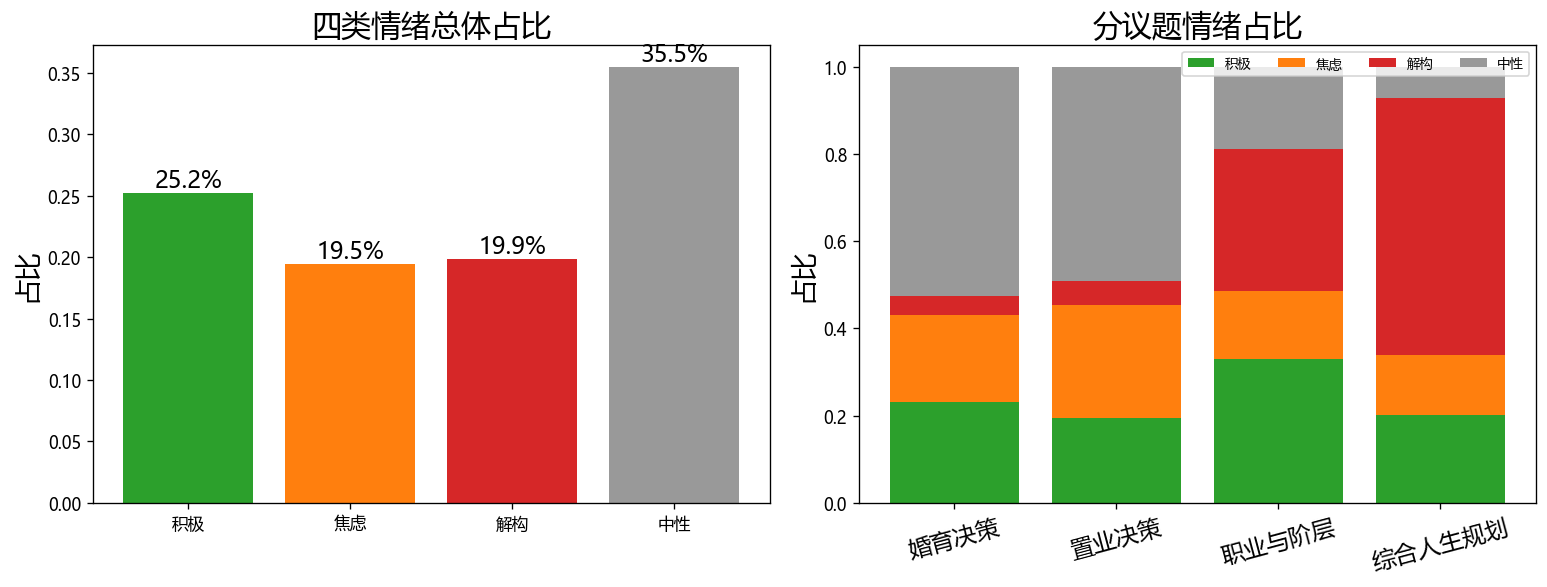
\includegraphics[width=0.62\textwidth]{emotion_dist.png}
  \caption{四类情绪的总体分布（$N=2503$）。}
  \label{fig:dist}
\end{figure}

季度演化（图~\ref{fig:trend}）显示，解构话语在 \textbf{2023Q1 出现占比高点（$\approx 0.48$）}，与"孔乙己文学"舆论事件的时点吻合；中性（信息型）话语在 2024--2025 年抬升至约 $0.38$。标志词曲线（图~\ref{fig:marker}）进一步佐证：躺平、摆烂、内卷的出现率随年份上行，梦想、奋斗、相信则走平或下行。但须强调，由于搜索接口偏向返回近期存量热门回答，时间序列反映的是"当下仍可见的存量话语"而非各时点全量发文，存在幸存者偏差。

\begin{figure}[H]
  \centering
  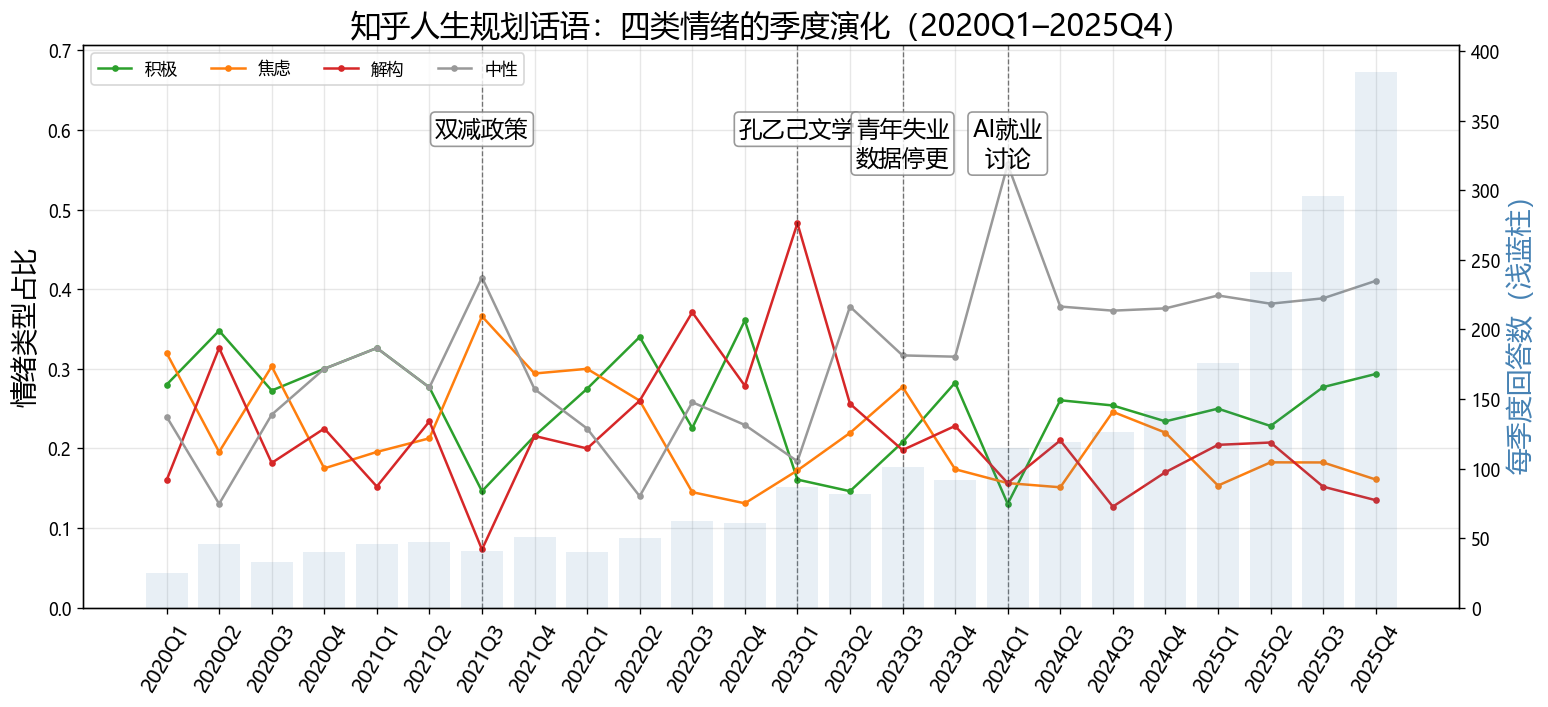
\includegraphics[width=0.85\textwidth]{emotion_trend.png}
  \caption{四类情绪占比的季度演化（2020Q1--2025Q4）。}
  \label{fig:trend}
\end{figure}

\begin{figure}[H]
  \centering
  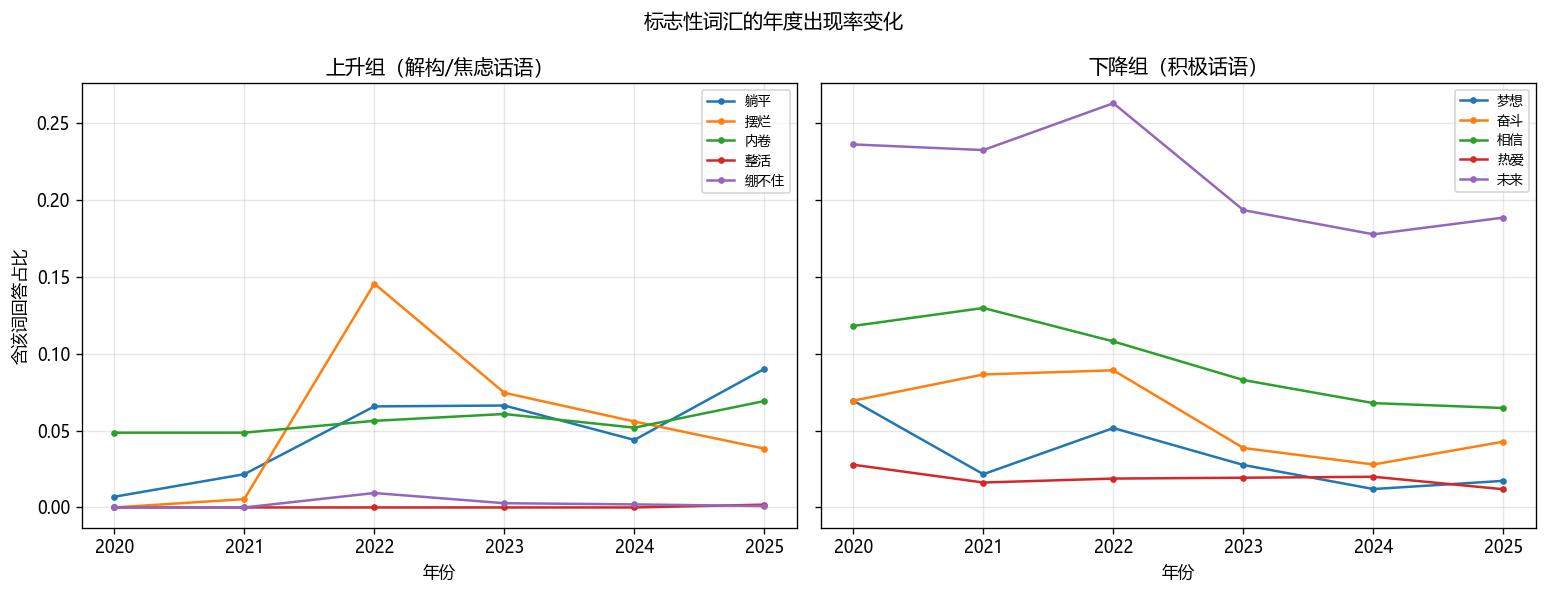
\includegraphics[width=0.78\textwidth]{marker_words.png}
  \caption{标志性词汇的年度出现率：上升组（躺平/摆烂/内卷）与下降组（梦想/奋斗/相信）。}
  \label{fig:marker}
\end{figure}

\subsection{情绪类型与传播效果（RQ2）}

主模型（式~\ref{eq:ols}，$N=2503$，$R^2=0.232$）结果见表~\ref{tab:ols}。控制变量符合预期：$\log$ 粉丝数（$\gamma_1 = 0.226$）与 $\log$ 长度（$\gamma_2 = 0.408$）均显著为正。核心结果有两层：

\begin{table}[H]
  \centering
  \small
  \caption{RQ2 主回归：情绪类型对 $\log(\text{赞同}+1)$ 的影响（参照组 $=$ 中性，HC1 稳健 SE）}
  \label{tab:ols}
  \begin{tabular}{lccccc}
    \toprule
    情绪（vs 中性） & 系数 $\beta$ & 标准误 & $p$ 值 & 95\% CI & 显著性 \\
    \midrule
    积极 & $-0.660$ & $0.112$ & $<0.001$ & $[-0.880,\,-0.440]$ & *** \\
    焦虑 & $-0.643$ & $0.118$ & $<0.001$ & $[-0.874,\,-0.412]$ & *** \\
    解构 & $-0.472$ & $0.136$ & $<0.001$ & $[-0.738,\,-0.206]$ & *** \\
    \midrule
    \multicolumn{6}{l}{\footnotesize 内部对比：解构$-$积极 $=+0.19$（$p=0.14$）；解构$-$焦虑 $=+0.17$（$p=0.22$）} \\
    \bottomrule
  \end{tabular}
\end{table}

\textbf{第一，三类情绪话语的获赞均显著低于中性/信息型话语}（$p<0.001$）。中性类多为长篇理性分析、"算账型"回答，在知乎获赞最高——这与"情绪化内容更易传播"的直觉\emph{相反}，但在四个稳健性设定（综合互动量、议题$\times$季度交互、高赞子样本）下符号一致，是稳健且可写的发现。

\textbf{第二，在情绪话语内部，解构类点估计最高}（$\beta=-0.47 > $ 积极 $-0.66$、焦虑 $-0.64$），方向上支持"解构传播优势"假说。但直接对比检验显示，解构$-$积极 $=+0.19$（$p=0.14$）、解构$-$焦虑 $=+0.17$（$p=0.22$），\textbf{均未达统计显著}。阈值敏感性分析表明，解构$-$积极的差异仅在中性占比 $\le 21\%$ 时才显著，而这些阈值对应的人工 Kappa 更低（$0.61$--$0.66$），故本文\emph{不主张}该显著性。

综上，本文最稳健的发现是"信息型理性话语获赞最高、情绪化话语普遍较低"；在情绪话语内部观察到\emph{解构话语的传播优势倾向}（方向一致但统计不显著）。这一结论比原假设更 nuanced，也更诚实。

\subsection{机制与因果稳健性（RQ3）}

\paragraph{事件研究 $+$ 双重差分。}
以 2023Q1"孔乙己文学"为外生冲击的 DiD（式~\ref{eq:did}，595 cell，37 关键词聚类）结果见图~\ref{fig:event}。事前各期交互系数约为 0 且置信区间包含 0，\textbf{平行趋势成立}。但 DiD 效应均不显著：解构话语占比 $\rho=+0.013$（$p=0.69$）、平均 $\log$ 赞同 $\rho=-0.469$（$p=0.13$）——未检出该事件的因果冲击，置信区间偏宽主要源于早期 cell 稀疏。

\begin{figure}[H]
  \centering
  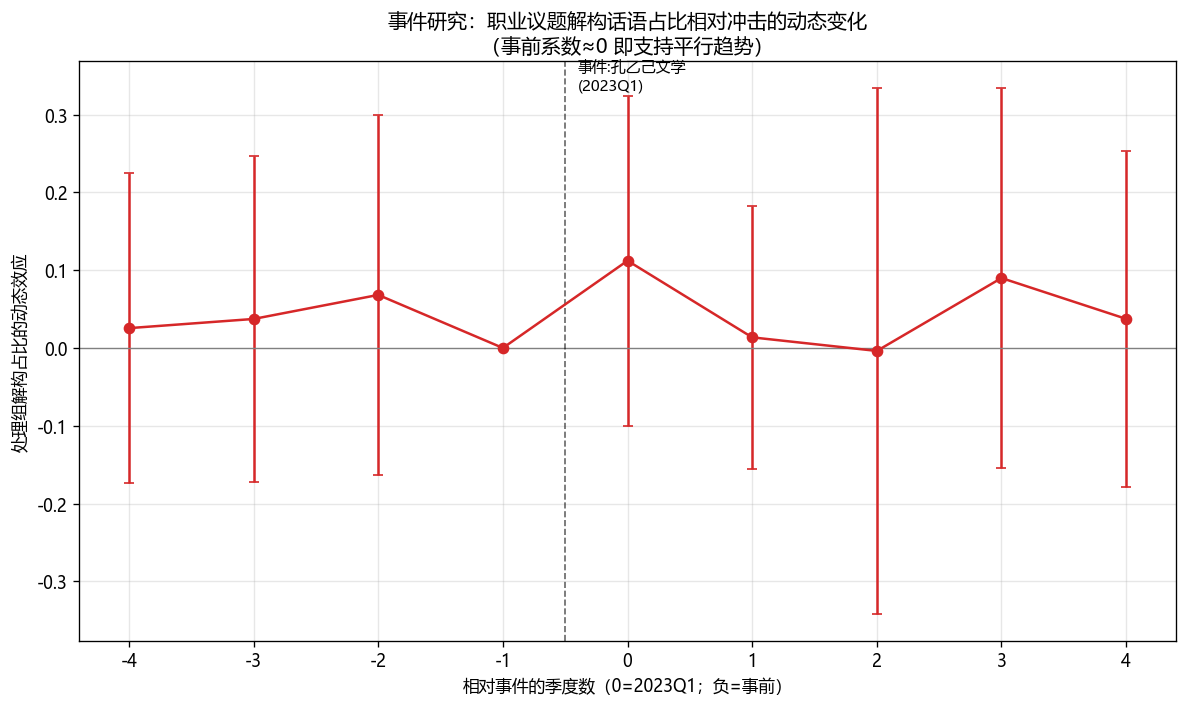
\includegraphics[width=0.82\textwidth]{event_study.png}
  \caption{以 2023Q1 为冲击点的事件研究：处理组（职业与阶层）相对对照组的逐期系数。}
  \label{fig:event}
\end{figure}

\paragraph{作者固定效应。}
在 188 位发文 $\ge 2$ 篇的作者子样本（$N=565$）上加入作者固定效应后，积极 $-0.181$（n.s.）、焦虑 $-0.733$（***）、解构 $-0.365$（*）。即在控制创作者个体后，"中性 $>$ 解构 $>$ 焦虑"的传播序仍然成立，说明 RQ2 的关联\textbf{并非仅由创作者构成造成}，而具有内容层面的来源。

%==================================================================
\section{讨论}

\subsection{对研究问题的回答}
本文能回答 RQ1（描述趋势）和 RQ2（关联性）：解构话语集中于人生规划/职业议题并在 2023Q1 出现高点；情绪话语获赞普遍低于中性话语，解构在情绪话语内部具有方向性优势。但本文\textbf{不能直接回答}"解构情绪导致传播"这一因果命题。

\subsection{关联背后的三种机制}
本文观察到的关联至少有三种并存的解释。\textbf{机制一（共鸣效应）}：解构内容击中青年真实情绪，产生"说出了我想说的话"的认同，从而获得更多赞同；这是内容驱动的解释，与作者固定效应下关联仍存在相一致。\textbf{机制二（算法正反馈）}：若平台推荐以互动为优化目标，而某类内容天然互动更高，算法会优先推送，形成正反馈，使情绪分布成为算法与用户偏好共同演化的结果。\textbf{机制三（创作者模仿）}：创作者观察到某种风格更受欢迎而主动迁移风格，使因果方向变为"互动反馈 $\rightarrow$ 话语分布"。三种机制并不互斥，本文的 OLS 回归无法在其间识别。

\subsection{因果识别的困难}
与课程核心方法（Angrist \& Pischke, 2009）对话，本文面临明显的\emph{遗漏变量偏误}（OVB）：宏观社会事件（如就业压力）可能同时影响创作者情绪倾向（自变量）与用户共鸣强度（因变量），导致 $\beta_k$ 有偏。本文已用事件研究、DiD 与作者固定效应作部分缓解，但 DiD 因早期样本稀疏、处理/对照划分基于研究者判断且议题级聚类数少，置信区间偏宽，未能提供决定性的因果证据。这恰恰说明：在缺乏外生变异与全量面板的观测数据上，从关联跨越到因果是困难的。

\subsection{研究局限}
（1）\emph{选择/幸存者偏误}：搜索接口返回近期存量热门回答，非时点全量发文，时间序列须谨慎解读。（2）\emph{因变量无浏览量}：以 $\log$ 赞同加曝光代理近似传播，并非真实互动率。（3）\emph{词典法对反讽弱}：$\kappa=0.78$ 但解构易与中性互混，解构效应可能被\emph{低估}，这反而使"解构无显著优势"成为偏保守的结论。（4）\emph{少聚类、处理分组非随机}：DiD 推断的统计功效有限。

%==================================================================
\section{结论}

本文基于知乎四类人生规划议题的 2503 条回答，量化刻画了优绩主义反叙事（解构话语）的分布、演化与传播效果。主要发现有三：其一，解构话语集中依附于综合人生规划与职业议题，并在 2023Q1"孔乙己文学"前后出现可见高点；其二，控制曝光与固定效应后，\textbf{信息型理性话语获赞最高、情绪化话语普遍较低}，这是本文最稳健的结论，与"情绪驱动传播"的直觉相反；其三，解构话语在情绪话语内部呈现方向性的传播优势，但未达统计显著，且事件研究与 DiD 未能提供因果证据。

在方法层面，本文展示了将情绪演化研究从质性观察推向量化验证的可行路径，也清晰呈现了因果推断框架在数字媒体研究中的应用边界——OVB、幸存者偏差与平台算法不透明共同构成识别障碍。在政策层面，若解构内容的传播优势部分由算法驱动，则推荐机制可能在无意中放大犬儒情绪的扩散，对理解青年心理健康的数字环境具有启示。未来研究可引入跨平台对比（知乎 vs B 站 vs 小红书）、寻找更干净的外生冲击以强化因果识别，并以预训练模型提升对反讽语境的识别精度。

%==================================================================
\section*{参考文献}
\begin{enumerate}[leftmargin=1.6em,itemsep=1pt,label={[\arabic*]}]
  \item Angrist, J.D. \& Pischke, J.S. (2009). \emph{Mostly Harmless Econometrics}. Princeton University Press.
  \item Kramer, A.D.I., Guillory, J.E., \& Hancock, J.T. (2014). Experimental evidence of massive-scale emotional contagion through social networks. \emph{PNAS}, 111(24), 8788--8790.
  \item Berger, J. (2011). Arousal increases social transmission of information. \emph{Psychological Science}, 22(7), 891--893.
  \item Brady, W.J., Wills, J.A., Jost, J.T., Tucker, J.A., \& Van Bavel, J.J. (2017). Emotion shapes the diffusion of moralized content in social networks. \emph{PNAS}, 114(28), 7313--7318.
  \item Sandel, M.J. (2020). \emph{The Tyranny of Merit: What's Become of the Common Good?} Farrar, Straus and Giroux.
  \item 徐琳宏, 林鸿飞, 潘宇, 等. (2008). 情感词汇本体的构造. \emph{情报学报}, 27(2), 180--185.
  \item Cohen, J. (1960). A coefficient of agreement for nominal scales. \emph{Educational and Psychological Measurement}, 20(1), 37--46.
\end{enumerate}

%==================================================================
\appendix
\section{附录}
\begin{itemize}[leftmargin=1.6em,itemsep=1pt]
  \item \textbf{附录 A}：四类情绪词典完整词表（积极 91 词、焦虑 99 词、解构 142 词），见 \texttt{analysis/lexicon/}。
  \item \textbf{附录 B}：RQ2 主模型完整系数表，见 \texttt{analysis/tables/rq2\_ols\_summary.txt}。
  \item \textbf{附录 C}：分类器人工校验与阈值敏感性，见 \texttt{tables/kappa.txt}、\texttt{classifier\_validation.csv}、\texttt{rq2\_threshold\_sensitivity.csv}。
  \item \textbf{复现}：全流程可由 \texttt{python -m analysis.run\_all} 复现。
\end{itemize}

\end{document}
